\documentclass[12pt]{report}

\usepackage{parskip}
\usepackage{graphicx}

\graphicspath{ {./images/} }
  
\begin{document}

1. Tell us a math joke.

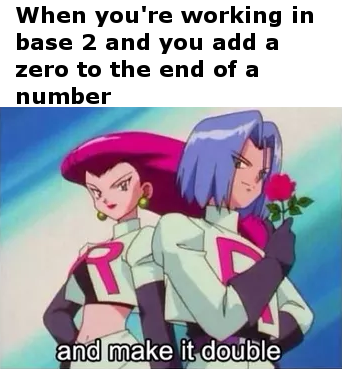
\includegraphics{math_joke}

\pagebreak

2a. Can you draw 5 points and connect each pair of points with a curve so that none of the curves touch except at their endpoints?


Not on a 2d plane.


2b. What rule am I using, to come up with this sequence? \\
\{1, 11, 21, 1211, 111221, 312211, 13112221, 1113213211, 31131211131221,...\}


You are taking how many times each number repeats before a different number repeats and converting that back into numeric form.


One $\rightarrow$ One one $\rightarrow$ Two ones $\rightarrow$ One two, One one, $\rightarrow$ One one, One two, Two ones $\rightarrow$ Three ones, Two twos, One one, and so forth.

\pagebreak


2c. What do you like about computer science?


Computer science is a manmade manifestation of magic in the world, and it makes me feel like a magician.
Its ability to break real-world applications down to chunks that bend to our every machination is unrivaled,
and in doing so brings us that much closer to being freed from the shackles that bind us to mindless work.

I also like watching my scripts run and stuff.

\end{document}